%------------------------------------------------------------------------------------
%	CHAPTER 2
%------------------------------------------------------------------------------------
\chapterimage{headerCap.jpeg}
\chapter{Quebrar a Cabeça}

\begin{remark}
	Você não é Assembly mas eu quebro muito a cabeça para te entender. (Davyd Maker) 
\end{remark}

\section{Aprendizado e desafios}\index{Quebrar a Cabeça}
Quando era mais jovem e iniciei no mundo da programação propus uma vez um desafia para mim, deveria fazer determinada coisa com a linguagem que escolhesse se conseguisse estava em bons caminhos, caso contrário, bem tentar novamente. Ou seja, era um desafio que não tinha muita saída, realizava ou realizava. Fosse ele fazer um programa para mostrar uma determinada figura na tela ou mesmo aprender a utilizar vetores. 

Ou seja fazia algo que muitas pessoas consideravam idiota (achou que ia falar impossível) e talvez realmente fosse, mas idiota no sentido de não ser algo prático para se utilizar, mas era meu modo de criar um "Hello World" mais inteligente. Nessa seção teremos meus quatro desafios básicos, e se posso quero lhe sugerir que tente resolvê-los antes de ler a solução. Veja qual é o desafio, entenda o requisito e resolva-o depois pode ver a solução. Vou lhe dar uma dica preciosa antes mesmo de começarmos, escreva no papel o que pretende fazer e organize suas ideias, senão conseguir organizá-las então isso não serve como programa.

Para todos os programas utilizaremos a biblioteca apenas com o conjunto do segmento data (de modo que possamos escrever os nomes e não os códigos) e o arquivo makefile para compilar e linkeditar, então se acostume a copiá-los para cada um dos programas descritos e que seja seu ponto de partida.

\section{Programa 10 - Quadrado}\index{Quebrar a Cabeça}
Com base em um determinado valor mostrar um quadrado de asteriscos. Como disse, as pessoas consideravam desafios idiotas pois nunca teremos um usuário pedindo: "Me dê um quadrado de asteriscos". Esse desafio é excelente para aprendermos a controlar estruturas de repetição determinada aninhas (vulgo comando "for" dentro de outro "for"). 
\begin{figure}[H]
	\centering
	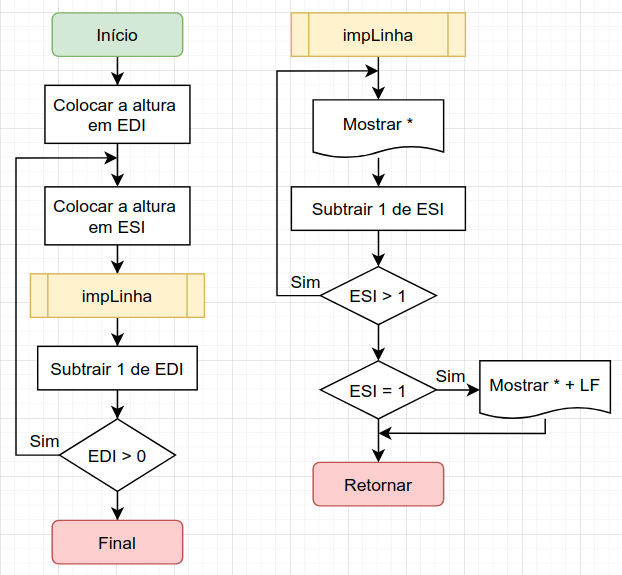
\includegraphics[width=0.6\textwidth]{Pictures/cap03/programa10}
	\caption{Fluxograma do Programa \textbf{Quadrado}}
\end{figure}

Vamos para o programa:

\begin{lstlisting}[]
%include 'bibliotecaE.inc'

SECTION .data
  estrela DB '*', LF, NULL
  altura EQU 4

SECTION .text

global _start
\end{lstlisting}

Começamos então com a definição da nossa cadeia de caracteres para a saída e do valor da altura. Vamos montar o corpo principal:

\begin{lstlisting}[]
_start:
  mov edi, altura

inicio:
  mov esi, altura
  call impLinha
  sub edi, 0x1
  cmp edi, 0x0
  je saida
  jmp inicio	
\end{lstlisting}

Colocamos o valor da altura em \textbf{EDI} (que controla a quantidade de linhas), para o marcador \textbf{inicio}, colocamos o valor da altura em \textbf{ESI} (que controla a quantidade de colunas), chamamos um método para mostrar 1 linha, reduzimos a quantidade de \textbf{EDI} e comparamos seu valor com 0, se for igual vamos para o marcador \textbf{saida} caso contrário retornamos para o marcador \textbf{início}.

\begin{lstlisting}[]
impLinha:
  call impEstrela
  sub esi, 0x1
  cmp esi, 0x1
  jg impLinha
  je impEstrelaFinal
  ret
\end{lstlisting}

No marcador \textbf{impLinha} mostramos um * na saída do terminal, reduzimos o valor de \textbf{ESI} e verificamos se este for maior que 1 retornamos para o marcador \textbf{impLinha}, se for igual mostramos "* + LF" (para saltar de linha) e retornamos para o ponto que nos chamou.

\begin{lstlisting}[]
saida:
  mov eax, SYS_EXIT
  mov ebx, EXIT_SUCESS
  int SYS_CALL	
\end{lstlisting}

Neste ponto apenas fazemos as movimentações para terminar o programa. Mas calma que ainda existem mais dois métodos importantes no conjunto.

\begin{lstlisting}[]
impEstrela:
  mov eax, SYS_WRITE
  mov ebx, STDOUT
  mov ecx, estrela
  mov edx, 0x1
  int SYS_CALL
  ret	
\end{lstlisting}

Observe que a cadeia de caracteres estrelas é formada por 3 elementos, dois deles é que nos interessam, se enviamos o tamanho em 1 apenas estamos tratando de mostrar '*' na saída do terminal e o cursor ficará na mesma linha, sem "cair" para a próxima.

\begin{lstlisting}[]
impEstrelaFinal:
  mov eax, SYS_WRITE
  mov ebx, STDOUT
  mov ecx, estrela
  mov edx, 0x2
  int SYS_CALL
  ret	
\end{lstlisting}

Já neste pedimos para mostrar o tamanho de dois que contém o '*' com Line Feed (ou quebra de linha se prefere) e assim ao mostrar o '*' desce para a próxima linha. Podemos agora imprimir quadrados de vários tamanhos, bastando apenas alterar a variável \textbf{altura}.

% Final do Capítulo
\clearpage